\documentclass{article}
\usepackage[utf8]{inputenc}
\usepackage[english]{babel}
\usepackage{setspace}
\usepackage{amssymb}
\usepackage{amsmath}
\usepackage{chngcntr}
\usepackage{float}
\usepackage{tabu}
\usepackage{bm}
\usepackage[lite]{amsrefs}
\usepackage{amsthm}
\usepackage{graphicx}
\usepackage{hyperref}\usepackage{xcolor}
%\graphicspath{ {./img/} }

\usepackage{graphicx}
\graphicspath{ {./images/} }

\usepackage{tikz}
\usetikzlibrary{matrix}


\newcommand{\shrug}[1][]{%
\begin{tikzpicture}[baseline,x=0.8\ht\strutbox,y=0.8\ht\strutbox,line width=0.125ex,#1]
\def\arm{(-2.5,0.95) to (-2,0.95) (-1.9,1) to (-1.5,0) (-1.35,0) to (-0.8,0)};
\draw \arm;
\draw[xscale=-1] \arm;
\def\headpart{(0.6,0) arc[start angle=-40, end angle=40,x radius=0.6,y radius=0.8]};
\draw \headpart;
\draw[xscale=-1] \headpart;
\def\eye{(-0.075,0.15) .. controls (0.02,0) .. (0.075,-0.15)};
\draw[shift={(-0.3,0.8)}] \eye;
\draw[shift={(0,0.85)}] \eye;
% draw mouth
\draw (-0.1,0.2) to [out=15,in=-100] (0.4,0.95); 
\end{tikzpicture}}




\counterwithin*{equation}{section}

\newcommand{\R}{\mathbb{R}}

\makeatletter
\newcommand*\bigcdot{\mathpalette\bigcdot@{1}}
\newcommand*\bigcdot@[2]{\mathbin{\vcenter{\hbox{\scalebox{#2}{$\m@th#1\bullet$}}}}}
\makeatother

\usepackage{afterpage}

\newcommand\blankpage{%
    \null
    \thispagestyle{empty}%
    \addtocounter{page}{-1}%
    \newpage}
    
\newtheorem{theorem}{Theorem}[section]
\newtheorem{definition}[theorem]{Definition}
\newtheorem{observation}[theorem]{Observation}
\newtheorem{corollary}{Corollary}[theorem]
\newtheorem{lemma}[theorem]{Lemma}

%\setlength{\parindent}{0pt}

\DeclareMathOperator*{\argmax}{\arg\!\max}
\DeclareMathOperator*{\argmin}{\arg\!\min}

\newcommand*{\defeq}{\mathrel{\vcenter{\baselineskip0.5ex \lineskiplimit0pt
                     \hbox{\scriptsize.}\hbox{\scriptsize.}}}%
                     =}

\usepackage[]{algorithm2e}


\newcommand*\OR{\ |\ }

\begin{document}


\title{NLP assignments \#1 and \# 2}
\author{Andrius Buinovskij - andriusb - 18-940-270}
\date{}

\maketitle

\section{Assignment \#1}

\textbf{Q1 a)}

	\includegraphics[angle=90,width=\textwidth]{comp_graph}

\textbf{Q1 b) i)}
	
	Well since all inputs are 1 and all weights are 1 then
	
	\begin{align}
		\mathbf{s}^1_1 &= \sum^3_{i=1} \mathbf{x}_i\cdot \mathbf{w}^1_{i, 1} = 3\\
		\mathbf{s}^1_2 &= \sum^3_{i=1} \mathbf{x}_i\cdot \mathbf{w}^1_{i, 2} = 3
	\end{align}
	
	Where $\mathbf{s}^i_j$ is the sum input to the $j$'th neuron in the $i$'th layer, and $\mathbf{s}^i$ is a vector whose length is equal to the number of neurons in the $i$'th layer, with the input being the $0$'th layer. So $\mathbf{s}^1$ is of length 2 since $1$'st layer has 2 neurons. 
	
	Let $\mathbf{n}^i_j$ be the output of the $j$'th neuron in the $i$'th layer, then of course $\mathbf{n}^i$ is a vector of length equal to the number of neurons in the $i$'th layer:
	
	\begin{align}
		n^i_j &= ReLU\big(\mathbf{s}^i_j\big)
	\end{align}
	
	So in our case We get
	
	\begin{align}
		\mathbf{n}^1_1 &= ReLU\big(\mathbf{s}^1_1\big) =  ReLU\big( 3 \big) = 3\\
	\mathbf{n}^1_2 &= ReLU\big(\mathbf{s}^1_2\big) =  ReLU\big( 3 \big) = 3	
	\end{align}
	
	Same steps in the next layer:
	
	\begin{align}
		\mathbf{s}^2_1 = 3\cdot 1 + 3\cdot 1 = 6
	\end{align}
	
	And now We pass this through a sigmoid for our output instead of a $ReLU$ so We get
	
	\begin{align}
		out = \sigma\big(\mathbf{s}^2_1)\big) = \frac{1}{1+e^{-6}} = 0.99752737684
	\end{align}


	
\textbf{Q1 b) ii-iv)}

	Alright let's just roll all of these questions into one and do an iteration of backprop.

	\begin{align}
		L_{BCE} &= -(y\log(\hat{y}) + (1-y)\log(1-\hat{y}))\\
		&= -(0\cdot\log(0.99752737684) + (1-0)\log(1-0.99752737684))\\
		&= -(\log(0.00247262316))\\
		&= 2.60684206722
	\end{align}
	
	The forward pass is trivial.
	
	Here is a pictorial view of the terms about to be defined:
	
	\includegraphics[angle=90,width=\textwidth]{notation_diagram}
	
	Let $\mathbf{x}^{l}_i$ be the output of the $i$'th neuron in the $l$'th layer. 
	
	Let $\mathbf{w}^l_{i, j}$ be the weight belonging to $j$'th neuron multiplying the $i$'th input in the $l$'th layer.  $\mathbf{w}^l_{.,j}$ is then simply the weight vector associated with the $j$'th neuron in the $l$'th layer.
	
	Let $\mathbf{s}^l_{j}$ be $(\mathbf{x}^{l-1})^\top\mathbf{w}^l_{.,j}$, the weighted sum of inputs to the $j$'th neuron in the $l$'th layer.
	
	We can then say that $x^l_i = \sigma(\mathbf{s}^l_j)$, where $\sigma$ is the nonlinearity of choice.
	
	Then define
	
	\begin{align}
		\delta^l_j = \frac{\partial L_{BCE}}{\partial \mathbf{s}^l_j}
	\end{align}
	
	And finally 
	
	\begin{align}
		\delta^{l-1}_j &= \sum^{d^l}_{i=1}\frac{\partial L_{BCE}}{\partial \mathbf{s}^l_i} \frac{\partial \mathbf{s}^l_i}{\partial \mathbf{x}^{l-1}_j}\frac{\partial \mathbf{x}^{l-1}_j}{\partial \mathbf{s}^{l-1}_j}\\
		&= \sum^{d^l}_{i=1}  \delta^l_i \frac{\partial \mathbf{s}^l_i}{\partial \mathbf{x}^{l-1}_j}\frac{\partial \mathbf{x}^{l-1}_j}{\partial \mathbf{s}^{l-1}_j}
	\end{align}
	
	Where $d^l$ is the number of neurons in layer $l$. So now We have a recursive definition which uses dynamic programming. This could be further nuanced by expressing things in matrix notation, but it's good enough for present purposes.
	
	
	 
	 So now taking the derivative of the loss w.r.t. first sum:
	 
	 \begin{align}
	 	\frac{\partial L_{BCE}}{\partial \mathbf{s}^2_1} = \frac{\partial L_{BCE}}{\partial \hat{y}} \frac{\partial \hat{y}}{\mathbf{s}^2_1} 
	 \end{align}
	 
	 Calculating terms individually:
	 
	 \begin{align}
	 	\frac{\partial L_{BCE}}{\partial \hat{y}} &= \frac{\partial }{\partial \hat{y}}-\big(y\log(\hat{y}) + (1-y)\log(1-\hat{y}) \big)\\
	 	&=-y\frac{1}{\hat{y}}  - (1-y)\frac{\partial }{\partial \hat{y}} \log(1-\hat{y}) \\
	 	&=-y\frac{1}{\hat{y}}  - (1-y)\frac{-1}{1-\hat{y}}\\
	 	&=-y\frac{1}{\hat{y}}  + \frac{1-y}{1-\hat{y}}
	 \end{align}
	 
	And the second bit in equation 15:
	 
	 \begin{align}
	 	\frac{\partial \hat{y}}{\mathbf{s}^2_1}  &= \frac{\partial }{\mathbf{s}^2_1} \sigma(\mathbf{s}^2_1)\\
	 	&= \sigma(\mathbf{s}^2_1)\cdot(1-\sigma(\mathbf{s}^2_1))
	 \end{align}
	 
	 So then We have 
	
	\begin{align}
	 	\delta^2_1 = \frac{\partial L_{BCE}}{\partial \mathbf{s}^2_1} &= \frac{\partial L_{BCE}}{\partial \hat{y}} \frac{\partial \hat{y}}{\mathbf{s}^2_1} \\
	 	&= \bigg( -y\frac{1}{\hat{y}}  + \frac{1-y}{1-\hat{y}} \bigg) \bigg( \sigma(\mathbf{s}^2_1)\cdot(1-\sigma(\mathbf{s}^2_1)) \bigg)
	 \end{align}
	 
	 Alright. We only have one more of these to figure out:
	 
	 \begin{align}
	 	\delta^1_j &= \sum^{d^2}_{i=1}  \delta^2_i \frac{\partial \mathbf{s}^2_i}{\partial \mathbf{x}^{1}_j}\frac{\partial \mathbf{x}^{1}_j}{\partial \mathbf{s}^{1}_j}
	 \end{align}
	 
	 
	 But since $d^2 = 1$, i.e. there is only one neuron in the output layer, We have

	\begin{align}
	 	\delta^1_j &= \sum^{d^2}_{i=1}  \delta^2_i \frac{\partial \mathbf{s}^2_i}{\partial \mathbf{x}^{1}_j}\frac{\partial \mathbf{x}^{1}_j}{\partial \mathbf{s}^{1}_j}\\
	 	&=   \delta^2_1 \frac{\partial \mathbf{s}^2_1}{\partial \mathbf{x}^{1}_j}\frac{\partial \mathbf{x}^{1}_j}{\partial \mathbf{s}^{1}_j}\\
	 	&=   \delta^2_1 \mathbf{w}^2_j \sigma(\mathbf{s}^{1}_j)(1-\sigma(\mathbf{s}^{1}_j))
	 \end{align}
	 
	 Now for the gradient update We will of course need
	 
	 \begin{align}
	 	\frac{\partial L_{BCE}}{\partial \mathbf{w}^l_{i, j}}
	 \end{align}
	 
	 But this can be easily derived since
	 
	 \begin{align}
	 	\frac{\partial L_{BCE}}{\partial \mathbf{w}^l_{i, j}} &= \frac{\partial L_{BCE}}{\partial \mathbf{s}^l_j}\frac{\partial \mathbf{s}^l_j}{\partial \mathbf{w}^l_{i, j}}\\
	 	&= \delta^l_j\mathbf{x}^{l-1}_i
	 \end{align}
	 
	 Now We do a forward pass and We know that $\mathbf{s}^1_i = 3$ and $\mathbf{s}^2_1 = 6$. Plugging in values We then get

	\begin{align}
	 	\delta^2_1 &= \bigg( -y\frac{1}{\hat{y}}  + \frac{1-y}{1-\hat{y}} \bigg) \bigg( \sigma(\mathbf{s}^2_1)\cdot(1-\sigma(\mathbf{s}^2_1)) \bigg)\\
	 	&= \bigg( \frac{1}{1-0.99752737684} \bigg) \bigg( \sigma(6)\cdot(1-\sigma(6)) \bigg)\\
	 	&= \bigg( \frac{1}{1-0.99752737684} \bigg) \bigg( 0.99752737684\cdot(1-0.99752737684) \bigg)\\
	 	&= 404.428792942\cdot 0.00246650929\\
	 	&= 0.99752737493
	 \end{align}
	 
	 Similarly We have
	 
	 \begin{align}
	 	\delta^1_j &=   \delta^2_1 \mathbf{w}^2_j \sigma(\mathbf{s}^{1}_j)(1-\sigma(\mathbf{s}^{1}_j))\\
	 	\delta^1_1 &=   \delta^2_1 \mathbf{w}^2_1 \sigma(\mathbf{s}^{1}_1)(1-\sigma(\mathbf{s}^{1}_1))\\
	 	&=   0.997527374931\cdot  \sigma(3)(1-\sigma(3))\\
	 	&=   0.997527374931\cdot  0.95257412682 \cdot 0.04742587317\\
	 	&= 0.04506495478
	 \end{align}
	 
	 $\delta^1_2$ is equal to $\delta^1_1$. 
	 
	 Now that We have the deltas We can use

	\begin{align}
	 	\frac{\partial L_{BCE}}{\partial \mathbf{w}^l_{i, j}} &= \delta^l_j\mathbf{x}^{l-1}_i
	 \end{align}
	 
	 For weights in the first layer this means

	\begin{align}
	 	\frac{\partial L_{BCE}}{\partial \mathbf{w}^1_{i, j}} &= \delta^1_j\mathbf{x}^{0}_i\\
	 	&= 0.04506495478\cdot 1\\
	 	&= 0.04506495478
	 \end{align}
	 
	 Where the 0'th layer is the input layer. 

	\begin{align}
	 	\frac{\partial L_{BCE}}{\partial \mathbf{w}^2_{i, j}} &= \delta^2_j\mathbf{x}^{1}_i\\
	 	&= 0.99752737493\cdot 3\\
	 	&= 2.99258212479
	 \end{align}
	 
	 All that is left is to perform a step for each weight. All weights in the first layer simplify to 
	 
	 \begin{align}
	 	w^1_{i, j} &= 1 - 0.1\cdot 0.04506495478\\
	 	&= 0.99549350452
	 \end{align}
	 
	 and similarly for the second layer:
	 
	  \begin{align}
	 	w^2_{i, j} &= 1 - 0.1\cdot 2.99258212479\\
	 	&= 0.70074178752
	 \end{align}
	 
	 \textbf{Sidenote}
	 
	 So when actually using this in the implementation of Q2, We get the following simplification:

	\begin{align}
	 	\delta^2_1 = \frac{\partial L_{BCE}}{\partial \mathbf{s}^2_1} &= \frac{\partial L_{BCE}}{\partial \hat{y}} \frac{\partial \hat{y}}{\mathbf{s}^2_1} \\
	 	&= \bigg( -y\frac{1}{\hat{y}}  + \frac{1-y}{1-\hat{y}} \bigg) \bigg( \sigma(\mathbf{s}^2_1)\cdot(1-\sigma(\mathbf{s}^2_1)) \bigg)\\
	 	&= \bigg( -y\frac{1}{\hat{y}}  + \frac{1-y}{1-\hat{y}} \bigg) \bigg(\hat{y}\cdot(1-\hat{y}) \bigg)\\
	 	&=  - \hat{y}\cdot(1-\hat{y})  \cdot \frac{y}{\hat{y}}  + \hat{y}\cdot(1-\hat{y}) \cdot \frac{1-y}{1-\hat{y}} \\
	 	&=  - (1-\hat{y})  \cdot y + \hat{y} \cdot (1-y)
	 \end{align}
	 
\textbf{Q1 c) )}

	Due to the fact that the weights were initialized as a uniform constant, I think that the second neuron in the hidden layer is redundant.
	
	I don't think We can get rid of the hidden layer all together due to the ReLU - if We simply passed the output of the sum to the sigmoid, the sigmoid could receive negative terms, which is not possible under the current architecture. As it is, the input to the sigmoid is bounded to be above zero regardless of the weights.
	
	The below is certainly more efficient and has fewer parameters:
	 
	 \includegraphics[angle=90,width=\textwidth]{redesign}
	 
	 The reason the $\times 2$ is there is to make the computation identical regardless of what the weights are initialized to, since currently the source of the redundancy is that the two neurons in the first hidden layer would output identical values.
	 
	 As for other benefits, numerical stability maybe?
	 
	 I don't think that this is the intended solution haha, but I don't think You can get rid of the hidden layer all together due to the ReLU as mentioned above, so \shrug
	 
	 
	 
\textbf{Q2}

	Running the script outputs the relevant comparisons.
	
	The scikit implementation performs slightly better, but the two are very comparable accuracy-wise e.g. 0.8925 0.8765 out-of-sample accuracy in the third test case.
	
	I should note that my implementation is almost an order of magnitude slower: prediction time sklearn: 0:00:00.000876 v.s. mine: 0:00:00.003137
	
	Finally, as can be seen by the output of the script, the sklearn implementation prefers smaller absolute values of the weights, where as my implementation does not seem shy about using larger values. Sklearn is superior in this regard.
	 

\newpage

\textbf{Q4 a) i)}

	We're going to use linearity of expectation.
	
	Let $I_i, i\in \{1\ldots |V|\}$ be the indicator variable for whether or not the word $i$ appears in Mary's sampling.
	
	Since draws are with replacement and the distribution is uniform, for a token \textit{not} to appear, all $n$ draws must have chosen another token. 
	
	The probability of not choosing token $i$ in a particular draw is of course $(|V|-1)/|V|$. The probability of not choosing token $i$ over $n$ samples is then
	
	\begin{align}
		\bigg(\frac{|V|-1}{|V|}\bigg)^n
	\end{align}
	
	However, We are interested in the opposite event - We want to know the probability of \textit{not} not choosing token $i$, which is given by
	
	\begin{align}
		1 - \bigg(\frac{|V|-1}{|V|}\bigg)^n
	\end{align}
	
	By linearity of expectation and the fact that the expected value of an indicator is simply the probability of it being 1, We get
	
	\begin{align}
		E\bigg(\sum^{|V|}_{i=1} = I_i \bigg) = \sum^{|V|}_{i=1} E(I_i) =  \sum^{|V|}_{i=1} P(I_i = 1) = |V|\cdot \bigg( 1 - \bigg(\frac{|V|-1}{|V|}\bigg)^n\bigg)
	\end{align}
	
\textbf{Q4 a) ii)}

	Given $n$ draws, what is the probability that all the words will appear in the sample? 
	
	All of my attempts have failed, and a whole lot of searching leads me to conclude that the probability is:
	
	\begin{align}
		\frac{|V|!}{|V|^n}S_2(n-1, |V|-1)
	\end{align}
	
	Where $S_2(n-1, |V|-1)$ is the Stirling number of the second kind. 
	
\textbf{Q4 b) i)}

	Alright, so, let $X$ be the number of samples before "work" and "hard" bigram appears.
	
	Let $ps$ (partial success) mean that the word "work" has been sampled. Then by law of total expectation We can say
	
	\begin{align}
		E(X) = (1+E(X|ps))\cdot P(ps) + (1+E(X|ps'))\cdot P(ps')
	\end{align}
	
	Where We the 1's in there come from the fact that a single sample has been taken.
	
	Now, given partial success We either fully succeed $(fs)$ or fail and go back to the beginning, so:
	
	\begin{align}
		E(X|ps) &= (1+E(X|ps, fs))\cdot P(fs|ps) + (1+E(X|ps, fs'))\cdot P(fs'|ps)\\
		&= (1)\cdot \frac{1}{|V|} + (1+E(X))\cdot \frac{|V|-1}{|V|}
	\end{align}
	
	Where given full success, expected number of draws to get a success is zero.  Given a failure We're back to $E(X)$.
	
	Of course, given $ps'$, the compliment of partial success i.e. partial failure, $E(X|ps') = E(X)$.
	
	Putting it all together We get:
	
	\begin{align}
		E(X) &= (1+E(X|ps))\cdot P(ps) + (1+E(X|ps'))\cdot P(ps')\\
		&= \bigg(1+\frac{1}{|V|} + (1+E(X))\cdot \frac{|V|-1}{|V|}\bigg)\cdot \frac{1}{|V|} + (1+E(X))\cdot \frac{|V| - 1}{|V|}\\
		&= \frac{1}{|V|}+\frac{1}{|V|^2} + (1+E(X))\cdot \frac{|V|-1}{|V|^2} + (1+E(X))\cdot \frac{|V|-1}{|V|}\\
		&= \frac{1}{|V|}+\frac{1}{|V|^2} + \frac{|V|-1}{|V|^2} + \frac{(|V|-1)E(X)}{|V|^2} + \frac{|V|-1}{|V|}+\frac{E(X)(|V|-1)}{|V|}
	\end{align}
	
	Now We just need to simplify this mess.
	
	\begin{align}
		&E(X) = \frac{1}{|V|}+\frac{1}{|V|^2} + \frac{|V|-1}{|V|^2} + \frac{(|V|-1)E(X)}{|V|^2} + \frac{|V|-1}{|V|}+\frac{E(X)(|V|-1)}{|V|}\\
		&E(X) - \frac{(|V|-1)E(X)}{|V|^2}-\frac{E(X)(|V|-1)}{|V|} = \frac{1}{|V|}+\frac{1}{|V|^2} + \frac{|V|-1}{|V|^2}  + \frac{|V|-1}{|V|}\\
		&E(X)\bigg(1 - \frac{(|V|-1)}{|V|^2}-\frac{(|V|-1)}{|V|}\bigg) = \frac{1}{|V|}+\frac{1}{|V|^2} + \frac{|V|-1}{|V|^2}  + \frac{|V|-1}{|V|}\\
		&E(X) = \frac{\frac{1}{|V|}+\frac{1}{|V|^2} + \frac{|V|-1}{|V|^2}  + \frac{|V|-1}{|V|}}{1 - \frac{(|V|-1)}{|V|^2}-\frac{(|V|-1)}{|V|}}
	\end{align}
	
	Beautiful. 
	
	For a sanity check, of You plug $|V|=2$ into that equation, You get 6, which is the well known result of expected number of tosses to get 2 heads in a row when tossing a fair coin, so it seems to work at least for that case.
	
	For an even further sanity check, I ran simulations for $|V|=1\ldots 10$, i.e. perform this experiment 100,000 times and check on average how many samples it took to receive two of the same word in a row given a uniform distribution, and for $|V|=1\ldots 10$, it's correct.
	
\textbf{Q4 b) ii)}

	Well, the probability of "work" not appearing in $n$ draws is
	
	\begin{align}
		\bigg( \frac{|V|-1}{|V|}\bigg)^n
	\end{align}
	
	And of course the probability of it appearing is
	
	\begin{align}
		1 - \bigg( \frac{|V|-1}{|V|}\bigg)^n
	\end{align}
	
	And Mary wants this probability to be above 0.95:

	\begin{align}
		1 - \bigg( \frac{|V|-1}{|V|}\bigg)^n &\ge 0.95\\
		- \bigg( \frac{|V|-1}{|V|}\bigg)^n &\ge -0.05\\
		\bigg( \frac{|V|-1}{|V|}\bigg)^n &\le 0.05\\
		\log\bigg(\bigg( \frac{|V|-1}{|V|}\bigg)^n\bigg) &\le \log(0.05)\\
		n\cdot\log\bigg( \frac{|V|-1}{|V|}\bigg) &\le \log(0.05)\\
		n &\ge \frac{\log(0.05)}{\log\big( \frac{|V|-1}{|V|}\big)}\\
	\end{align}
	
	Where the last sign flips since log of a quantity less than 1 is negative. 

\textbf{Q4 c) i)}

	The answer here is identical to the answer to question \textbf{b)i)}, by the fact that the tokens are all equally likely.
	
	
\textbf{Q4 c) ii)}

	Okay so We have
	
	\begin{align}
		h^0_t = f(w_0x_{t-1} + w_1 x_t + w_2h^0_{t-1} + b_0)
	\end{align}
	
	So, that's our first hidden state. $f$ is some arbitrary non-linearity (or maybe linearity, whatever, a function).
	
	$w_0$ multiplies previous input, $w_1$ multiplies current input, $w_2$ multiplies the previous hidden state and We have a bias term. 
	
	The output then is
	
	\begin{align}
		y_t = g(w_3h^0_t + b_1)
	\end{align}
	
	So $w_3$ is multiplying the hidden state, there's a bias  term and another function. 
	
	The goal is to output 1 if $x_{t-1}$ and $x_t$ are the same word.
	
	Okay so assume that  the two words are equal and the bias is 0:
	
	\begin{align}
		h^0_t &= f(w_0x_{t-1} + w_1 x_t + w_2h^0_{t-1} + b_0)\\
		&= f(w_0x_{t-1} + w_1 x_{t-1})\\
		&= f(x_{t-1}(w_0+w_1))
	\end{align}
	
	So clearly one way to go is to let $w_0$ be -1 and $w_1$ be 1, so that when they are added, We get zero in the case of equality. Then $f$ can just be like a check as to whether the input is 0, and if it is output 1, otherwise output 0.
	
	$g$ is then simply the identity function and $b_1$ is also 0.
	
	So, $w_0 = -1$, $w_1 = 1$, $w_2 = 0$, $w_3=1$, all biases are zero, $f$ is a boolean check for whether the input is $0$ and $g$ is the identity function.
	
\textbf{Q4 c) iii)}	

	So We simply use the second hidden layer as a counter. $w_4, w_5=1$, $b_1, b_2 = 0$ and $g$ and $h$ are still the identity function, and $f$ is the boolean 0 check.	

\textbf{Q4 c) iv)}		
	
	I think the non-uniform unigram language model has the greater probability of drawing two of the same token in a row. 
	
	This isn't a proof, but the reasoning is as follows: let $p_i$ be the probability of drawing the $i$'th token. Now suppose We alter the distribution such that $p_i' = p_i - x$. Now, We'll have to add that $x$ to some other $p_j$ to preserve a distribution, and since the sample are identical, sampling $p_j$ twice in a row will be more likely than if We had just left the probabilities alone.
	
	
\newpage

\textbf{Q5 a) i)}

	For the person correcting this: below is a re-derivation of semiring thing. If You'd like to skip it, scroll down until You see \textbf{stop scrolling}. I left the work in since, well, I did it, and so if something went wrong in the derivation, You can at least see what led to the error.

	Well first let's re-derive this mess.
	
	\begin{align}
		\sum_{\mathbf{t}\in\mathcal{T}^N} \exp\bigg\{ \sum^N_{n=1} \text{score}\big( \langle t_{n-1}, t_n \rangle, \mathbf{w} \big) \bigg\}
	\end{align}	
	
	So let's start with inside the bracket comes from
	
	\begin{align}
		\text{score}\big(\mathbf{t}, \mathbf{w} \big) = \sum^N_{n=1} \text{score}\big( \langle t_{n-1}, t_n \rangle, \mathbf{w} \big)
	\end{align}
	
	So this is our simplifying assumption, and I suppose it's also what makes this a "Conditional Random Field". $\mathbf{t}$ stands for "tag" and it's the, well, tagging of the word sequence $\mathbf{w}$. So We're saying that the score for  the tag does not have to be calculated all in one go, but rather can be done in parts, where each part only depends on it's predecessor. 
	
	$N$ is the length of the sentence by the way, so the length of both $\mathbf{t}$ and $\mathbf{w}$. 
	
	$\mathcal{T}$ is the set of all possible tags for any particular word. Since there are $N$ words, the total number of possible tags for $\mathbf{w}$ is then $\mathcal{T}^N$.
	
	So then the expression is simply calculating the normalizing constant, since it's summing over all possible tags $\mathbf{t}\in\mathcal{T}^N$.
	
	So, up next We get
	
	\begin{align}
		&\sum_{\mathbf{t}\in\mathcal{T}^N} \exp\bigg\{ \sum^N_{n=1} \text{score}\big( \langle t_{n-1}, t_n \rangle, \mathbf{w} \big) \bigg\}\\
		&= \sum_{\mathbf{t}_{1:n}\in\mathcal{T}^N} \prod^N_{n=1} \exp \big\{ \text{score}(\langle \mathbf{t}_{n-1}, \mathbf{t}_n \rangle, \mathbf{w}) \big\}
	\end{align}	
	
	Okay so what have We done here. For one, $\mathbf{t}$ now has a subscript. Sure.
	
	We've converted the inner sum to a product, which is fine - before We were taking the exponent of a sum, but product of a bunch of exponents will sum the exponents so no worries there. We then still sum over every possible tag. Sure. 
	
	\begin{align}
		&\sum_{\mathbf{t}\in\mathcal{T}^N} \exp\bigg\{ \sum^N_{n=1} \text{score}\big( \langle t_{n-1}, t_n \rangle, \mathbf{w} \big) \bigg\}\\
		&= \sum_{\mathbf{t}_{1:n}\in\mathcal{T}^N} \prod^N_{n=1} \exp \big\{ \text{score}(\langle \mathbf{t}_{n-1}, \mathbf{t}_n \rangle, \mathbf{w}) \big\}\\
		&= \sum_{\mathbf{t}_{1:N-1}\in\mathcal{T}^{N-1}} \sum_{t_N\in \mathcal{T}} \prod^N_{n=1} \exp \big\{ \text{score}(\langle \mathbf{t}_{n-1}, \mathbf{t}_n \rangle, \mathbf{w}) \big\}
	\end{align}	
	
	So, the first change is that the subscript for $\mathbf{t}$ now goes to $N-1$. So We're just taking out the last tag in the sequence of tags $\mathbf{t}_N$.
	
	Since that last tag could be anything, We sum over all the possible tags, so $t_N\in\mathcal{T}$. There are $|\mathcal{T}|$ choices.
	
	I mean really You could rewrite the first sum as $N$ sums each over $|\mathcal{T}|$ terms each. So We're just splitting one out. No worries.
	
	\begin{align}
		&\sum_{\mathbf{t}\in\mathcal{T}^N} \exp\bigg\{ \sum^N_{n=1} \text{score}\big( \langle t_{n-1}, t_n \rangle, \mathbf{w} \big) \bigg\}\\
		&= \sum_{\mathbf{t}_{1:n}\in\mathcal{T}^N} \prod^N_{n=1} \exp \big\{ \text{score}(\langle \mathbf{t}_{n-1}, \mathbf{t}_n \rangle, \mathbf{w}) \big\}\\
		&= \sum_{\mathbf{t}_{1:N-1}\in\mathcal{T}^{N-1}} \sum_{t_N\in \mathcal{T}} \prod^N_{n=1} \exp \big\{ \text{score}(\langle \mathbf{t}_{n-1}, \mathbf{t}_n \rangle, \mathbf{w}) \big\}\\
		&= \sum_{\mathbf{t}_{1:N-1}\in\mathcal{T}^{N-1}} \prod^{N-1}_{n=1} \exp \big\{ \text{score}(\langle \mathbf{t}_{n-1}, \mathbf{t}_n \rangle, \mathbf{w}) \big\} \times \sum_{t_N\in\mathcal{T}} \exp \big\{ \text{score}(\langle \mathbf{t}_{N-1}, \mathbf{t}_N \rangle, \mathbf{w}) \big\}
	\end{align}	
	
	Okay so if I had to explain this in words, how would I do it?
	
	Well, everything hinges on two parts - the first being that the score can be decomposed into partial computations. If there is no substructure, no simplification is possible. 
	
	The second I suppose is the distributative property I suppose. The key bit is that You can take stuff out of the product and sum it, and if You take the product of the stuff and the sum it all still works. Or rather, You have some operator $B$. $B$ is iterating over all possible versions of the tags. Then You also have some operator $A$, and You can take stuff out of $B$, combine it with $A$ and take output of $A$ and stick it back into $B$ and it all still works. Now You're reducing the exponential number of things You had to deal with. Sure.
	
	Another way of saying it is that $A$ has to give You the ability to group and it has to work with $B$ via distributativity.
	
	The viterbi algorithm just keeps track of max possible value for each node going backwards using multiplication and max. 
	
	Vertices $V$ are the tags, edges $E$ are pairs of tags, and the weight on each tag would be score($a, b$). These should really be directed in our case but it ought to work regardless.
	
	\textbf{stop scrolling}
	
	\begin{algorithm}[H]
		 \KwData{Graph, source node}
		 \KwResult{Shortest path from source to all nodes}
		 prq = initialize priority queue with source node with distance 0\;
		 //scores is a dictionary of tuples such that \\
	 	//scores[a] = (b, c) where c is  the cumulative score of a\\
	 	//and c is the node We took to arrive at a with score c\\
		 scores = empty dictionary\;
		 //initialize scores to include source node
		 scores[source] = (source, 1)\;
		 \While{prq not empty}{
		 	//popMin retrieves and removes minimum entry in prq\\
		 	//the minimum is decided by the associated score\\
		 	//see prq.add below\\
		 	currentNode = prq.popMax() \;
		 	\For{neighbour in neighbours(currentNode)}{
		 		//scores[neighbour](1) accesses the tuple for\\
		 		//neighbour and (1) accesses the cumulative score\\
		 		tempScore = scores[neighbour](1) + score(neighbour, currentNode)\\
		 		\If{tempScore $>$ score[neighbour]}{
		 			scores[neighbour] = (currentNode, tempScore)\\
		 			//tempScore is what is used to rank the options\\
		 			//and prq returns the neighbour entry \\
		 			//when popMax is called\\
		 			//loops will not enter prq due to increasing score\\
		 			//and anyway the graph We care about is acyclic\\
		 			prq.add(neighbour, tempScore)
		 		} 
		 	}
		}
		 \caption{Dijsktra's algorithm using a priority queue.}
	\end{algorithm}
	
	To get the best path, one simply picks the node they would like to find the path from, find the node in the scores list, look at it's predecessor, then look at the predecessor of the predecessor and so on.
	
\textbf{Q5 a) ii)}

	Well the algorithm will visit every node once, so it's $\mathcal{O}(|V|)$ for that. 
	
	It'll also examine every edge twice - let $a, b,$ be nodes, then it will look at the edge $(a, b)$ first and sometime later at the edge $(b, a)$, so $2|E|$ there or $\mathcal{O}(|E|)$. In those cases it will also consult the priority queue $prq$, and the complexity of that in the best case\footnote{With Fibonacci heaps.}  is $\log(|V|)$, so in total We get $\mathcal{O}(|E|\cdot\log(|V|) + |V|)$.
	
	In contrast, Viterbi visits each edge and node once, so We have $\mathcal{O}(|V| + |E|)$ time complexity. This obviously compares favourably with Dijsktra.
	
	Now, since Dijsktra explores more promising venues first, it is possible to construct examples where, despite being worse asymptotically, Dijsktra will beat Viterbi. 
	
	Likewise one could construct examples where Viterbi will beat Dijsktra. Neither is strictly better than the other, but Viterbi is better on average.
	
\textbf{Q5 b) i)}

	Well first let's identify the semiring.
	
	$A$ are strictly positive real numbers of course.
	
	$\bigoplus$ is the $\max$ operation. 
	
	$\bigotimes$ is the $\times$ operation, i.e. just simple multiplication. This works due to the fact that We're exponentiating, so taking the product leads to the sum in the exponent We want.
	
	$\hat{0}, \hat{1}$ are 0 and 1 respectively.
	
	In semiring notation We then get an algorithm that looks basically nothing like the first version:
	
	\begin{algorithm}[H]
		 \KwData{Graph $G$, score function, source node s}
		 \KwResult{Shortest path from source to all nodes}
		prq = initialize max queue with source node and score of 1\;
		scores = dictionary initialized with source node and value of 1\;
		 \caption{Dijsktra's algorithm using a priority queue in semiring notation.}
		 \While{Q not empty}{
			currentNode = prq.popMax()\;
			\For{each neighbour of currentNode}{
				tempScore = score[neighbour] $\bigoplus \big($scores(currentNode) $\bigotimes$ score(neighbour) $\big)$\;
				\If{scores[neighbour](1) $<$ tempScore}{
					//scores[neighbour]= parent, new best score\\
					scores[neighbour] =(currentNode, tempScore)\;
					//priority decided based on score obviously\\
					prq.add(neighbour, tempScore)\;
				}
			}
		 }
	\end{algorithm}
	
	It's a little different since I don't like initializing the queue with the entire graph at the beginning. Instead, the queue is initialized with just the source and entries are added as You go. This could be dicey in cyclic settings, but We don't have to worry about cycles in our case. Don't think I'd use this with a cyclic graph, since cycles would just continue increasing the score and get continuously added.
	
	To get the path one traverses the parents in scores, same as before - each node has a parent, and to get the path You take the parent of the goal node, then the parent of the parent and so on.
	
\textbf{Q5 b) ii)}
	
	I think just using $\bigoplus = \min$ operation should work, and of course the priority queue would now use popMin instead of popMax, and also the if condition changes to $>$. I think this would not work in general due to cycles, but our graph is acyclic. 
	
\textbf{Q5 b) iii)}

	Well, I think the $\bigotimes = \min$, since given a path We'll want to take the minimum out of all the edge values.
	
	Could You use $\bigoplus = \max$? I think that's it. Across an entire path We want to take the minimum to find the minimal value, but when choosing amongst a number of possible edges to take, We'll choose the maximum. 
	
\newpage
\section{Assignment \# 2}

\textbf{Q1 a)}

	\begin{align}
		S &\to NP, VP\\
		NP &\to Det, N \OR NP, PP \OR "I" \OR "glasses"\\
		VP &\to VP, PP \OR V, NP\\		
		Det &\to "a" \OR "an"\\
		N &\to "man" \OR "pencil" \OR "ball" \OR "umbrella"\\
		PP &\to P, NP\\
		V &\to "draw" \OR "hit"\\
		P &\to "with" 
	\end{align}
	
\textbf{Q1 b)}

	Warning: advanced calculations ahead (instead of probabilities We just do counts first):

	\begin{align}
		S &\to NP, VP (4)\\
		NP (14) &\to Det, N (7) \OR NP, PP (2)\OR "I" (4)\OR "glasses" (1)\\
		VP (6)&\to VP, PP (2)\OR V, NP (4)\\		
		Det (7)&\to "a" (6) \OR "an"(1)\\
		N (7)&\to "man" (4)\OR "pencil"(1) \OR "ball"(1) \OR "umbrella"(1)\\
		PP (4)&\to P, NP (4)\\
		V (4)&\to "draw" (2) \OR "hit"(2)\\
		P (4)&\to "with" (4) 
	\end{align}
	
	Convert to probabilities (rounded, for precise figures just divide counts on the right by total counts on the left):
	
	\begin{align}
		S &\to NP, VP (1.0)\\
		NP  &\to Det, N (0.5) \OR NP, PP (0.14)\OR "I" (0.29)\OR "glasses" (0.7)\\
		VP (&\to VP, PP (2=0.33)\OR V, NP (0.66)\\		
		Det &\to "a" (0.86( \OR "an"(0.14)\\
		N &\to "man" (0.57)\OR "pencil"(0.14) \OR "ball"(0.14) \OR "umbrella"(0.14)\\
		PP &\to P, NP (1)\\
		V &\to "draw" (0.5) \OR "hit"(0.5)\\
		P &\to "with" (1) 
	\end{align}
	
\textbf{Q1 c)}

	Our goal is to have different likelihood of expansions on noun phrase depending on whether the expansion is going to be an object or a subject.

	I suppose a logical way of going about it would be to replace the noun phrase non-terminal with two other non terminals - object phrase ($OP$) and subject phrase ($SP$). 
	
	\begin{align}
		S &\to NP, VP (1.0)\\
		NP &\to SP \OR  OP\\
		SP &\to Det, N (0.5) \OR NP, PP (0.14)\OR "I" (0.29)\OR "glasses" (0.7)\\
		OP &\to Det, N (0.5) \OR NP, PP (0.14)\OR "I" (0.29)\OR "glasses" (0.7)\\
		VP (&\to VP, PP (2=0.33)\OR V, NP (0.66)\\		
		Det &\to "a" (0.86( \OR "an"(0.14)\\
		N &\to "man" (0.57)\OR "pencil"(0.14) \OR "ball"(0.14) \OR "umbrella"(0.14)\\
		PP &\to P, NP (1)\\
		V &\to "draw" (0.5) \OR "hit"(0.5)\\
		P &\to "with" (1) 
	\end{align}
	
	Here are the counts as before:
	
	\begin{align}
		S &\to NP, VP (1.0)\\
		NP (14)&\to SP (4)\OR  OP (10)\\
		SP (4) &\to Det, N (0) \OR NP, PP (0)\OR "I" (4) \OR "glasses" (0)\\
		OP (10)&\to  Det, N (7) \OR NP, PP (2)\OR "I" (0)\OR "glasses" (1)\\
		VP (&\to VP, PP (2=0.33)\OR V, NP (0.66)\\		
		Det &\to "a" (0.86( \OR "an"(0.14)\\
		N &\to "man" (0.57)\OR "pencil"(0.14) \OR "ball"(0.14) \OR "umbrella"(0.14)\\
		PP &\to P, NP (1)\\
		V &\to "draw" (0.5) \OR "hit"(0.5)\\
		P &\to "with" (1) 
	\end{align}
	
	Finally converting to probabilities:
	
	\begin{align}
		S &\to NP, VP (1.0)\\
		NP &\to SP (0.29)\OR  OP (0.71)\\
		SP (4) &\to Det, N (0) \OR NP, PP (0)\OR "I" (1) \OR "glasses" (0)\\
		OP (10)&\to  Det, N (0.7) \OR NP, PP (0.2)\OR "I" (0)\OR "glasses" (0.1)\\
		VP (&\to VP, PP (2=0.33)\OR V, NP (0.66)\\		
		Det &\to "a" (0.86( \OR "an"(0.14)\\
		N &\to "man" (0.57)\OR "pencil"(0.14) \OR "ball"(0.14) \OR "umbrella"(0.14)\\
		PP &\to P, NP (1)\\
		V &\to "draw" (0.5) \OR "hit"(0.5)\\
		P &\to "with" (1) 
	\end{align}
	
	Well this at least shows that subject phrases are likely to be "I", and object phrases are unlikely to be "I", so it's capturing some of what We wanted to. 
	
	There is a problem here of course - nothing is stopping anyone from using $SP$ instead of $OP$ wherever they like, so the onus is on the user of the grammar to use the subject non-terminal for subjects and the object non-terminal for objects.
	
\textbf{Q1 d)}
	
	\begin{align}
		S &\to NP, VP^+\\
		NP &\to Det, N^+ \OR NP^+, PP \OR "I" \OR "glasses"\\
		VP &\to VP^+, PP \OR V^+, NP\\		
		Det &\to "a" \OR "an"\\
		N &\to "man" \OR "pencil" \OR "ball" \OR "umbrella"\\
		PP &\to P, NP^+\\
		V &\to "draw" \OR "hit"\\
		P &\to "with" 
	\end{align}
	
	\includegraphics[angle=90,origin=c,width=\textwidth]{figures/headed_parse_tree}
	
	
	
\textbf{Q2 a)}

	So, it is my understanding that for the projective dependency tree, to obtain the score We would simply take all dependency pairs and multiply the scores corresponding to those dependencies (taking care to pay attention to the direction of the dependency etc.)
	
	To obtain the score of a lexicalized probabilistic context free grammar tree, one also simply multiplies the score for each "rule" applied, except this rule is also lexicalized so You have very many parameters indeed (page 15 from \href{http://www.cs.columbia.edu/~mcollins/courses/nlp2011/notes/lexpcfgs.pdf}{\_ click me\_}.)
	
	With all that out of the way, I would construct a weighted lexicalized CFG as follows: 
	
	1. Add root productions $R \to X_j$, $j\in 1\ldots M$.
	
	2. Add self-productions $X_j \to j$.
	
	3. For each production $\psi(i\to j)$, add bidirectional productions to the language as follows:
	
	\begin{align}
		X_i \to X_i^+, X_j\\
		X_i \to X_j, X_i^+
	\end{align}
	
	And of course they weight for that transformation corresponds to the value of $\psi(i\to j)$ does not You anything about the ordering of words within a sentence.
	
	The reason for adding bidirectional rules is that just having access to the set of weights generated by 
	
	And that's all She wrote.
	
\textbf{Q2 b)}

	So the dependency tree would simply be $ROOT\to fish$, $fish\to they$, and the score would be $\psi(ROOT, fish)\cdot \psi(fish, they)$.
	
	In our CFG We would end up with $ROOT\to S$, then $S\to NP$, 
	
	\includegraphics[angle=90,origin=c,width=\textwidth]{figures/relational_parse}
	

	
\newpage
\textbf{Q4 a)}

	\begin{table}[ht]
        \centering
        \fontsize{10}{10}\selectfont
        \renewcommand{\arraystretch}{1.2} % vertical padding
        \setlength{\tabcolsep}{0.5em} % for the horizontal padding
        \begin{tabular}{l|l|l|l}
        \textbf{number} & \textbf{sample strings} & \textbf{accepted} & \textbf{weight} \\ \hline
        1 & educational is this not & NO &  \\
        2 & is this assignment educational & NO & \\
        3 & not educational is not educational  & YES & 12 \\
        4 & this assignment is not educational & YES & 7 \\
        5 & is this assignment educational & NO &  \\
        6 & this assignment course is educational & NO  &  \\
        7 & is this assignment not educational &  YES & 15 \\
        8 & this assignment not & YES & 8 \\
        9 & this course assignment is not educational & YES  & 12 \\
        10 & this course is not not educational & YES & 21 \\
        11 & not educational is this & YES & 10 \\
        12 & course assignment is not educational & YES & 10 \\
        13 & not this assignment is educational & NO &  \\
        14 & not not not educational & YES & 25 \\
        15 & is this course assignment not educational  & YES & 18 \\
        16 & course assignment is this & YES & 8 \\
        17 & this course is interesting & NO &  \\
        18 & this course assignment not educational & YES & 14
        \end{tabular}
        \caption{Some strings from $\mathcal{Y}_{\geq 2, \leq 6}$}
        \label{tab:wfst_strings}
        \end{table}
	
	
\textbf{Q4 b)}

	Cost matrices on left, backtracking matrices on the right.
	
	"inf" means an infinite cost, i.e. no path exists, and similarly "N" in the backtracking matrix means a backtrack is not possible.
	
Iteration 0

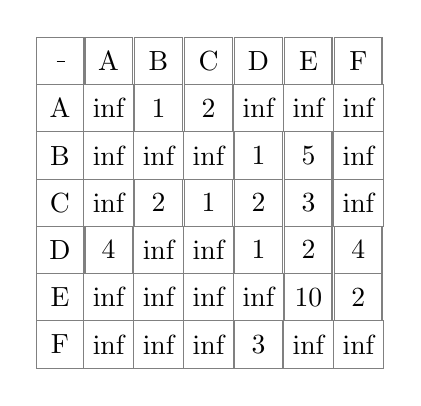
\begin{tikzpicture}
\matrix[matrix of nodes,nodes={draw=gray, anchor=center, minimum size=.6cm}, column sep=-\pgflinewidth, row sep=-\pgflinewidth] (A) {
 &\_ & A & B & C & D & E & F \\ & A & inf & 1 & 2 & inf & inf & inf\\
 & B & inf & inf & inf & 1 & 5 & inf\\
 & C & inf & 2 & 1 & 2 & 3 & inf\\
 & D & 4 & inf & inf & 1 & 2 & 4\\
 & E & inf & inf & inf & inf & 10 & 2\\
 & F & inf & inf & inf & 3 & inf & inf\\
};
\end{tikzpicture}
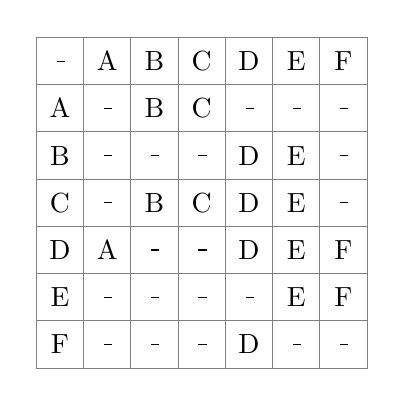
\begin{tikzpicture}
\matrix[matrix of nodes,nodes={draw=gray, anchor=center, minimum size=.6cm}, column sep=-\pgflinewidth, row sep=-\pgflinewidth] (A) {
 &\_ & A & B & C & D & E & F \\ & A & \_ & B & C & \_ & \_ & \_\\
 & B & \_ & \_ & \_ & D & E & \_\\
 & C & \_ & B & C & D & E & \_\\
 & D & A & \_ & \_ & D & E & F\\
 & E & \_ & \_ & \_ & \_ & E & F\\
 & F & \_ & \_ & \_ & D & \_ & \_\\
};
\end{tikzpicture}


Iteration 1

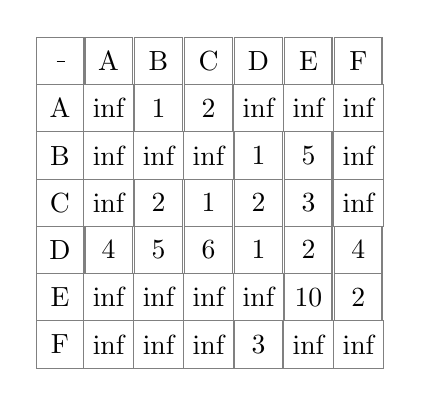
\begin{tikzpicture}
\matrix[matrix of nodes,nodes={draw=gray, anchor=center, minimum size=.6cm}, column sep=-\pgflinewidth, row sep=-\pgflinewidth] (A) {
 &\_ & A & B & C & D & E & F \\ & A & inf & 1 & 2 & inf & inf & inf\\
 & B & inf & inf & inf & 1 & 5 & inf\\
 & C & inf & 2 & 1 & 2 & 3 & inf\\
 & D & 4 & 5 & 6 & 1 & 2 & 4\\
 & E & inf & inf & inf & inf & 10 & 2\\
 & F & inf & inf & inf & 3 & inf & inf\\
};
\end{tikzpicture}
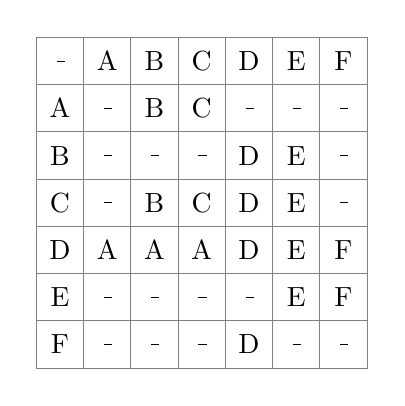
\begin{tikzpicture}
\matrix[matrix of nodes,nodes={draw=gray, anchor=center, minimum size=.6cm}, column sep=-\pgflinewidth, row sep=-\pgflinewidth] (A) {
 &\_ & A & B & C & D & E & F \\ & A & \_ & B & C & \_ & \_ & \_\\
 & B & \_ & \_ & \_ & D & E & \_\\
 & C & \_ & B & C & D & E & \_\\
 & D & A & A & A & D & E & F\\
 & E & \_ & \_ & \_ & \_ & E & F\\
 & F & \_ & \_ & \_ & D & \_ & \_\\
};
\end{tikzpicture}


Iteration 2

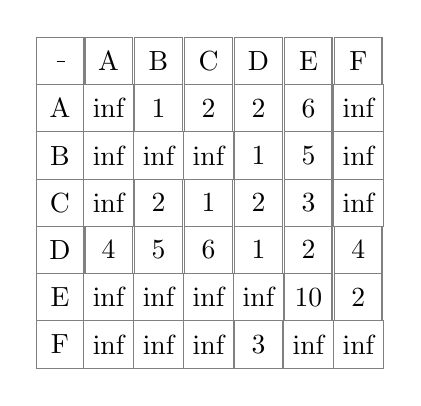
\begin{tikzpicture}
\matrix[matrix of nodes,nodes={draw=gray, anchor=center, minimum size=.6cm}, column sep=-\pgflinewidth, row sep=-\pgflinewidth] (A) {
 &\_ & A & B & C & D & E & F \\ & A & inf & 1 & 2 & 2 & 6 & inf\\
 & B & inf & inf & inf & 1 & 5 & inf\\
 & C & inf & 2 & 1 & 2 & 3 & inf\\
 & D & 4 & 5 & 6 & 1 & 2 & 4\\
 & E & inf & inf & inf & inf & 10 & 2\\
 & F & inf & inf & inf & 3 & inf & inf\\
};
\end{tikzpicture}
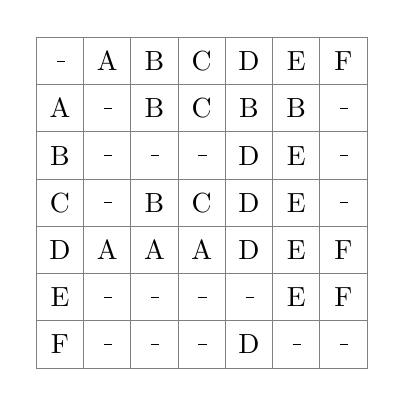
\begin{tikzpicture}
\matrix[matrix of nodes,nodes={draw=gray, anchor=center, minimum size=.6cm}, column sep=-\pgflinewidth, row sep=-\pgflinewidth] (A) {
 &\_ & A & B & C & D & E & F \\ & A & \_ & B & C & B & B & \_\\
 & B & \_ & \_ & \_ & D & E & \_\\
 & C & \_ & B & C & D & E & \_\\
 & D & A & A & A & D & E & F\\
 & E & \_ & \_ & \_ & \_ & E & F\\
 & F & \_ & \_ & \_ & D & \_ & \_\\
};
\end{tikzpicture}


Iteration 3

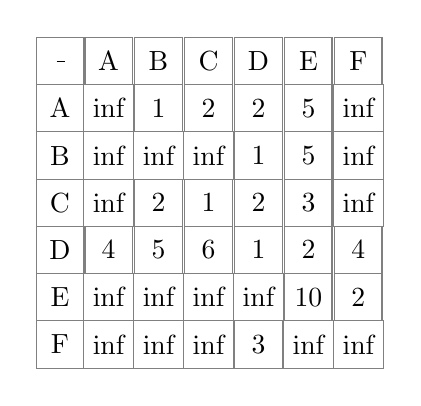
\begin{tikzpicture}
\matrix[matrix of nodes,nodes={draw=gray, anchor=center, minimum size=.6cm}, column sep=-\pgflinewidth, row sep=-\pgflinewidth] (A) {
 &\_ & A & B & C & D & E & F \\ & A & inf & 1 & 2 & 2 & 5 & inf\\
 & B & inf & inf & inf & 1 & 5 & inf\\
 & C & inf & 2 & 1 & 2 & 3 & inf\\
 & D & 4 & 5 & 6 & 1 & 2 & 4\\
 & E & inf & inf & inf & inf & 10 & 2\\
 & F & inf & inf & inf & 3 & inf & inf\\
};
\end{tikzpicture}
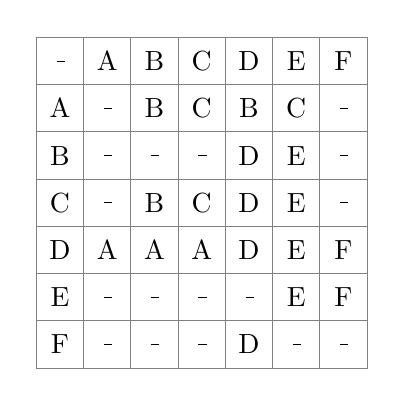
\begin{tikzpicture}
\matrix[matrix of nodes,nodes={draw=gray, anchor=center, minimum size=.6cm}, column sep=-\pgflinewidth, row sep=-\pgflinewidth] (A) {
 &\_ & A & B & C & D & E & F \\ & A & \_ & B & C & B & C & \_\\
 & B & \_ & \_ & \_ & D & E & \_\\
 & C & \_ & B & C & D & E & \_\\
 & D & A & A & A & D & E & F\\
 & E & \_ & \_ & \_ & \_ & E & F\\
 & F & \_ & \_ & \_ & D & \_ & \_\\
};
\end{tikzpicture}


Iteration 4

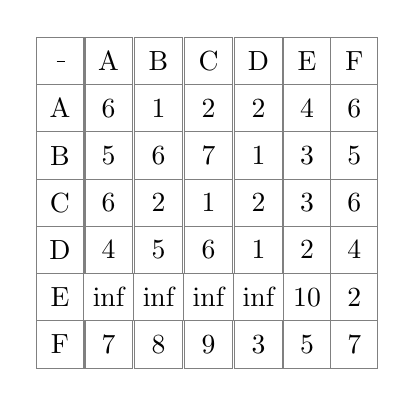
\begin{tikzpicture}
\matrix[matrix of nodes,nodes={draw=gray, anchor=center, minimum size=.6cm}, column sep=-\pgflinewidth, row sep=-\pgflinewidth] (A) {
 &\_ & A & B & C & D & E & F \\ & A & 6 & 1 & 2 & 2 & 4 & 6\\
 & B & 5 & 6 & 7 & 1 & 3 & 5\\
 & C & 6 & 2 & 1 & 2 & 3 & 6\\
 & D & 4 & 5 & 6 & 1 & 2 & 4\\
 & E & inf & inf & inf & inf & 10 & 2\\
 & F & 7 & 8 & 9 & 3 & 5 & 7\\
};
\end{tikzpicture}
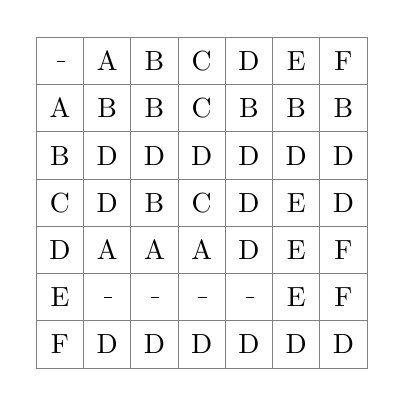
\begin{tikzpicture}
\matrix[matrix of nodes,nodes={draw=gray, anchor=center, minimum size=.6cm}, column sep=-\pgflinewidth, row sep=-\pgflinewidth] (A) {
 &\_ & A & B & C & D & E & F \\ & A & B & B & C & B & B & B\\
 & B & D & D & D & D & D & D\\
 & C & D & B & C & D & E & D\\
 & D & A & A & A & D & E & F\\
 & E & \_ & \_ & \_ & \_ & E & F\\
 & F & D & D & D & D & D & D\\
};
\end{tikzpicture}


Iteration 5

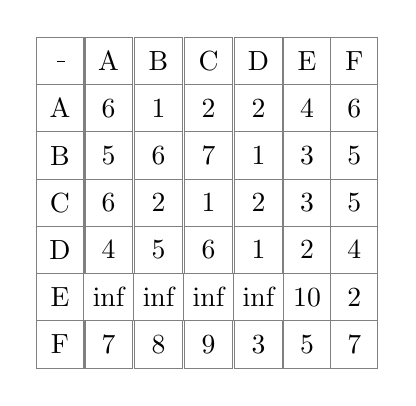
\begin{tikzpicture}
\matrix[matrix of nodes,nodes={draw=gray, anchor=center, minimum size=.6cm}, column sep=-\pgflinewidth, row sep=-\pgflinewidth] (A) {
 &\_ & A & B & C & D & E & F \\ & A & 6 & 1 & 2 & 2 & 4 & 6\\
 & B & 5 & 6 & 7 & 1 & 3 & 5\\
 & C & 6 & 2 & 1 & 2 & 3 & 5\\
 & D & 4 & 5 & 6 & 1 & 2 & 4\\
 & E & inf & inf & inf & inf & 10 & 2\\
 & F & 7 & 8 & 9 & 3 & 5 & 7\\
};
\end{tikzpicture}
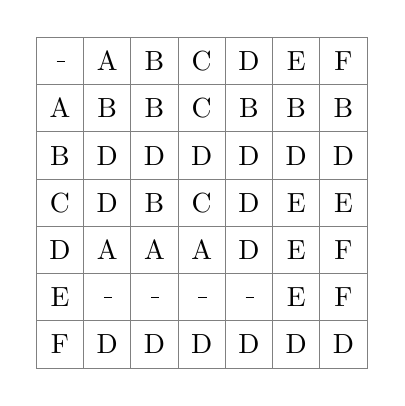
\begin{tikzpicture}
\matrix[matrix of nodes,nodes={draw=gray, anchor=center, minimum size=.6cm}, column sep=-\pgflinewidth, row sep=-\pgflinewidth] (A) {
 &\_ & A & B & C & D & E & F \\ & A & B & B & C & B & B & B\\
 & B & D & D & D & D & D & D\\
 & C & D & B & C & D & E & E\\
 & D & A & A & A & D & E & F\\
 & E & \_ & \_ & \_ & \_ & E & F\\
 & F & D & D & D & D & D & D\\
};
\end{tikzpicture}

Final 6th iteration

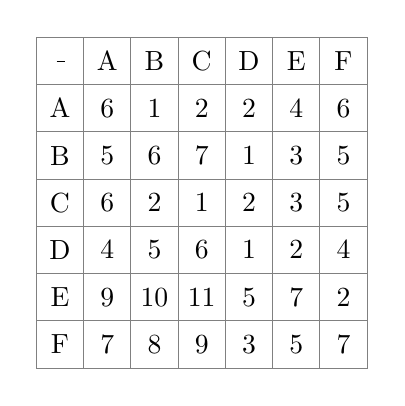
\begin{tikzpicture}
\matrix[matrix of nodes,nodes={draw=gray, anchor=center, minimum size=.6cm}, column sep=-\pgflinewidth, row sep=-\pgflinewidth] (A) {
 &\_ & A & B & C & D & E & F \\ & A & 6 & 1 & 2 & 2 & 4 & 6\\
 & B & 5 & 6 & 7 & 1 & 3 & 5\\
 & C & 6 & 2 & 1 & 2 & 3 & 5\\
 & D & 4 & 5 & 6 & 1 & 2 & 4\\
 & E & 9 & 10 & 11 & 5 & 7 & 2\\
 & F & 7 & 8 & 9 & 3 & 5 & 7\\
};
\end{tikzpicture}
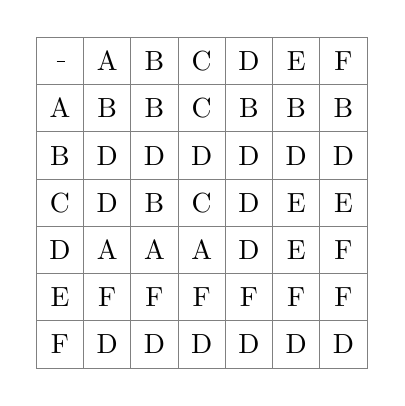
\begin{tikzpicture}
\matrix[matrix of nodes,nodes={draw=gray, anchor=center, minimum size=.6cm}, column sep=-\pgflinewidth, row sep=-\pgflinewidth] (A) {
 &\_ & A & B & C & D & E & F \\ & A & B & B & C & B & B & B\\
 & B & D & D & D & D & D & D\\
 & C & D & B & C & D & E & E\\
 & D & A & A & A & D & E & F\\
 & E & F & F & F & F & F & F\\
 & F & D & D & D & D & D & D\\
};
\end{tikzpicture}
	
\textbf{Q4 c)}

	The number of iterations is bound by $\mathcal{O}(N^3)$, where $N$ is the number of nodes. 
	
	The algorithm terminated after 6 iterations, so after looking at all of the nodes.
	
\textbf{Q4 d)}
	
	The time complexity is $\mathcal{O}(N^3)$ and for the method I used the space complexity is $N^2$. Strictly speaking it's more like $4N^2$ since I was keeping new and old versions of matrices around in my implementation, but this can be reduced. Asymptotically, it's simply $\mathcal{O}(N^2)$ for space complexity and $\mathcal{O}(N^3)$ for time complexity.
	
	Backtracking takes $\mathcal{O}(n)$ and is achieved as follows: let starting node be $u$ and ending node be $v$. Now take the $v$'th column of the backtracking matrix, and begin at the $u$'th entry. The value of the $u$'th entry is the next node in the shortest path. Then simply follow the entries until the desired destination is reached. 
	
	This makes sense intuitively - it may be the case that to go from $u$ to $v$ one has to traverse all the nodes, but no node should be traversed more than once since if it were, then there is a cycle in the path that could be cut out.
	
\end{document} 